\section{Raycasting}

\subsection{Direct Volume Rendering}

Volume rendering (sometimes called \emph{direct volume rendering}) stands for methods that generate images directly from $3$D scalar data. "Directly" means: \emph{no intermediate geometry} (such as an isosurface) is 
generated.

Volume rendering techniques
\begin{itemize}
    \item Depend strongly on the grid type.
    \item Exist for structured and unstructured grids.
    \item Are predominantly applied to uniform grids with $2$D or $3$D image data with \emph{cell-centered} data.
    Cell-centered data 
    \begin{itemize}
        \item are attributed to cells (pixels, voxels) rather than nodes,
        \item can also occur in (finite volume) CFD datasets,
        \item are converted to node data:
            \begin{itemize}
                \item By taking the \emph{dual grid} (easy for uniform grids: $n$ cells $\rightarrow$ $n-1$ cells!),
                \item or by interpolating. 
            \end{itemize}
    \end{itemize}
\end{itemize}


\subsection{Raycasting}
\emph{Raycasting} is historically the first volume rendering technique. It is very similar to \emph{raytracing}:
\begin{itemize}
    \item \emph{image-space} method: The main loop iterates over the pixels of the output image,
    \item a \emph{view ray} per pixel (or per subpixel) is traced backward,
    \item and samples are taken along the ray and \emph{composited} to a single color.
\end{itemize}
The differences are
\begin{itemize}
    \item No secondary (reflected, shadow) rays,
    \item the transmitted ray is not refracted,
    \item more elaborate compositing functions,
    \item and samples are taken at intervals (not at object intersections).
\end{itemize}

\subsubsection{Compositing}
Two simple compositing functions can be used for previewing:
\begin{description}
    \item[Maximum intensity projection] (MIP):
        \begin{itemize}
            \item Maximum of sampled values
            \item Result resembles X-ray image.
        \end{itemize}
    \item[Local maximum Intensity projection] (LMIP):
        \begin{itemize}
            \item Choose first local maximum which is above a prescribed threshold.
            \item Process approximates occlusion.
            \item It is faster and better than MIP.
        \end{itemize}
        \begin{figure}[H]
            \centering
            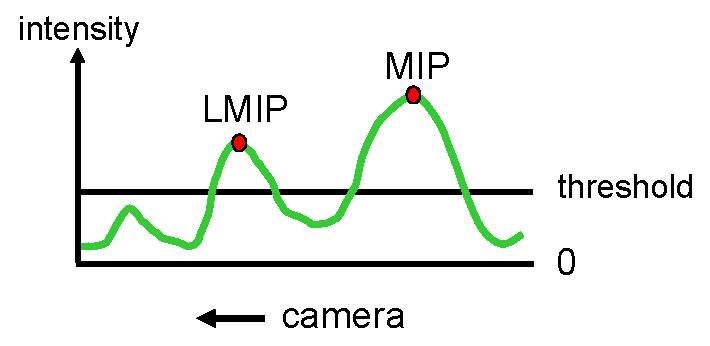
\includegraphics[width=0.6\textwidth]{img/03_lmip}
        \end{figure}
\end{description}

\subsubsection{$\alpha$-compositing}
Assume that each sample on a view ray has a \emph{color} and \emph{opacity}.
\begin{align*}
    (C_0,\alpha_0), \ldots, (C_N,\alpha_N)\qquad\qquad C_i\in [0,1]^3,\ \ \alpha_i\in [0,1]
\end{align*}
where the $0^{th}$ sample is next to the camera and the $N^{th}$ one is a (fully opaque) background sample:
\begin{align*}
    C_N &= (r,g,b)_\text{background}\\
    \alpha_N &= 1.
\end{align*}
$\alpha$-compositing can be defined recursively:

Let $C_f^b$ denot the \emph{composite color} of samples $f$, $f+1$, $\ldots$, $b$. The recursion formula for \emph{back-to-front} compositing yields:
\begin{align*}
    C_b^b &= \alpha_b C_b\\
    C_f^b &= \alpha_f C_f + (1-\alpha_f)C_{f+1}^b.
\end{align*}
With \emph{transparency} set to $T_i = 1-\alpha_i$ we get a \emph{closed formula} for $\alpha$-compositing:
\begin{align*}
    C_f^b = \sum_{i=f}^b \alpha_i C_i \prod_{j=f}^{j-1} T_j
\end{align*}
The \emph{front-to-back} compositing can be derived from the closed formula: Let $T_f^b$ denote the \emph{composite transparency} of samples $f$, $f+1$, $\ldots$, $b$:
\begin{align*}
    T_f^b = \prod_{j=f}^b T_j.
\end{align*}
Then the \emph{simultaneous recursion} for front-to-back composition is:
\begin{align*}
    C_f^f &= \alpha_f C_f\\
    T_f^f &= 1-\alpha_f\\
    C_f^{b+1} &= C_f^b + \alpha_{b+1} C_{b+1} T_f^b\\
    T_f^{b+1} &= (1-\alpha_{b+1})T_f^b.
\end{align*}

\paragraph{The emission-absorption model} How realistic is $\alpha$ compositing? The \emph{emission-absorption} model (Sabella 1988) yields a basic \emph{volume rendering equation}"
\begin{align*}
    L(x) = \int_x^{x_b} \varepsilon (x') \exp\left( -\int_x^{x'} \tau (x'') dx''\right) dx'
\end{align*}
The equation describes the \emph{radiance} arriving along a ray at the position $x$ on this ray. The \emph{emission} function $\varepsilon(x)$ describes the photons "emitted" by the volume along the ray. The \emph{absorbtion} function $\tau(x)$ is the probability that that photon traveling over a unit distance is lost by absorption.


The emission-absorption model is based on the Boltzmann transport equation in statistical physics, but completely \emph{ignores scattering}. In more general models $\tau(x)$ is an \emph{extinction function} having both an absorption term and a scattering term.

Instead, in the emission-absorption model:
\begin{itemize}
\item \emph{Incident scattering} is modelled by the emission function
\item \emph{Loss by scattering} can be thought to be part of the absorption.
\end{itemize}


The discrete version of the emission absorption model:
\begin{align*}
    L(x) = \sum_{i=0}^n \varepsilon_i \Delta x \exp\left( -\sum_{j=0}^{i-1} \tau_j \Delta x \right) 
    = \sum_{i=0}^n \varepsilon_i \Delta x\prod_{j=0}^{i-1} e^{- \tau_j \Delta x},
\end{align*}
matches the $\alpha$-compositing formula
\begin{align*}
    C_f^b = \sum_{i=f}^b \alpha_i C_i \prod_{j=f}^{j-1} (1-\alpha_i)
\end{align*}
and gives interpretations of "opacity" and "color":
\begin{align*}
    \alpha_i &= 1-e^{\tau_j\Delta x} \approx \tau_j \Delta x &\text{if }\Delta x << 1\\
    \alpha_i C_i &= \varepsilon_i \Delta x.
\end{align*}

The product $\tilde C = \alpha_i C_i$ is called a \emph{premultiplied} or \emph{associated} colour.

\subsection{Transfer Functions}
\emph{Transfer functions} map raw voxel data to opacities and colours as needed for the $\alpha$-compositing. Inputs of the TF (one or more):
\begin{itemize}
    \item Voxel value $s(x)$
    \item Gradient magnitude $\norm{\nabla s(x)}$
    \item Higher derivatives of $s(x)$.
\end{itemize}

\begin{description}
\item \emph{Opacity transfer function} $\alpha(s(x), \norm{\nabla s(x)}, \ldots)$
\item \emph{Color transfer function} $C(s(x), \norm{\nabla s(x)}, \ldots)$
\end{description}

In general TF don't depend on \emph{spatial location}, exception for \emph{focus and context} techniques.

By choosing different opacity transfer functions different types of applications can be achieved.
\begin{figure}[H]
\centering
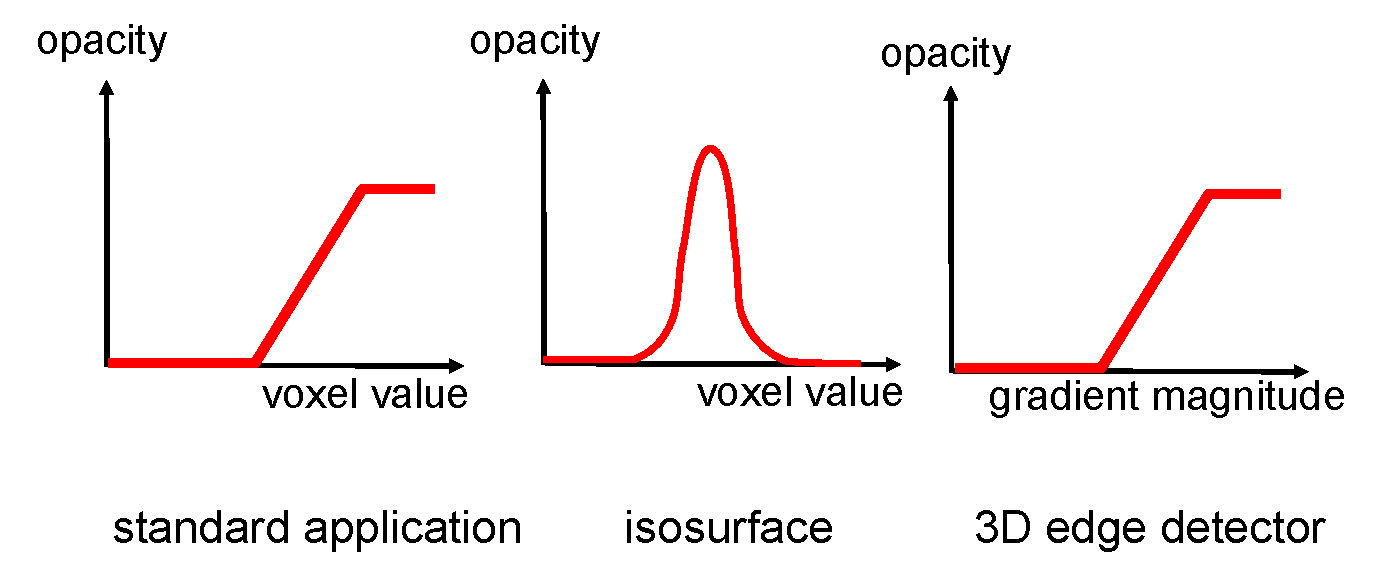
\includegraphics[width=0.8\textwidth]{img/03_tf_types}
\end{figure}

Example of a \emph{bivariate} (=2D) transfer function:
\begin{figure}[H]
    \centering
    \includegraphics[width=0.6\textwidth,page=1]{img/03_tf_bivariate}
\end{figure}
Example of a bivariate transfer function for an isosurface of constant thickness.
\begin{figure}[H]
    \centering
    \includegraphics[width=0.6\textwidth,page=2]{img/03_tf_bivariate}
\end{figure}

The color transfer function allows to make a simple \emph{classification}.
\begin{figure}[H]
    \centering
    \includegraphics[width=0.8\textwidth,page=1]{img/03_tf_color}
\end{figure}

\paragraph{Pre-classification} In pre-classification, the voxels can also be lit:
\begin{itemize}
    \item The gradient is perpendicular to the local isosurface. It can be used as a normal vector for \emph{Phong lighting} (without rendering the isosurface itself).
    \item \emph{Reflection coefficients} can be assigned by a separate transfer function ("materials" instead of only colors).
    \item \emph{Diffuse lighting} can be applied to the entire volume dataset as a pre-processing since it's independent of the viewing direction.
\end{itemize}

\subsubsection{Pre- vs. Post-classification}
For quality reasons, current volume rendering implementations often use \emph{post-classficiation}.

\begin{description}
\item[Pre-Classification] $\ $
    \begin{enumerate}
        \item Transfer functions are applied to voxels.
        \item Results are interpolated to sample locations.
    \end{enumerate}
\item[Post-Classification] $\ $
    \begin{enumerate}
        \item Raw data are interpolated to sample locations.
        \item Transfer functions are applied to sampled data.
    \end{enumerate}
\end{description}

\subsection{Preintegration}
Idea (Engel 2001): Simulate \emph{infinitely many} interpolated samples between two successive samples $s_i= s(x_i)$ and $s_{i+1} = s(x_{i+1})$. Assuming that 
\begin{itemize}
    \item Field $s(x)$ varies \emph{linearly} between samples
    \item and that the transfer functions don't depend on derivatives.
\end{itemize}

The discrete formula for opacity at a sample was
\begin{align*}
    \alpha_i = 1-e^{-\tau_i \Delta x}.
\end{align*}
The continuous version for a sample interval $[x_i, x_{i+1}]$ is 
\begin{align*}
    \alpha_i = 1-e^{-\int_{x_i}^{x_{i+1}} \tau(s(x)) dx}.
\end{align*}
Assuming now $s(x)$ to be linear between samples, we get:
\begin{align*}
    \alpha_i &= 1-\exp\left( {-{d\over s_{i+1}-s_i} \int_{s_i}^{s_{i+1}}\tau(s) ds}\right) &\text{with } d= \norm{x_{i+1}-x_i}, 
\end{align*}
which is called a \emph{preintegrated opacity transfer function}.


The integral
\begin{align*}
\int_{s_i}^{s_{i+1}} \tau(s) ds = \int_0^{s_{i+1}} \tau(s) ds - \int_0^{s_i} \tau(s)ds
\end{align*}
can be evaluated by two lookups in a precomputed table of 
\begin{align*}
\int_0^{s} \tau(s')ds'.
\end{align*}

The composite colour of the same interval
\begin{align*}
  C_i = \int_{x_i}^{x_{i+1}} \varepsilon (s(x))\exp\left(-\int_{x_i}^x \tau(s(x'))dx'\right) dx,
\end{align*}
simplifies for linear $s(x)$ to:
\begin{align*}
  C_i = {d\over {s_{i+1}-s_i}} \int_{s_i}^{s_{i+1}} \varepsilon (s)\exp\left(-{d\over {s_{i+1}-s_i}} \int_{s_i}^x \tau(s')ds'\right) ds,
\end{align*}
which can be precomputed for all combinations of $s_i$, $s_{i+1}$ and $d$.

\subsubsection{Extinction-based volume rendering}
Instead of an opacity Transfer function, use an extinction TF [Schlegel 2011]. Advantage: Extinction is \emph{additive}.
\begin{itemize}
    \item Riemann sums for numerical integration give better accuracy.
    \item Additivity can be used for efficient lighting.
\end{itemize}

\paragraph{Screen-Space ambient occlusion} Approximate the fraction of ambient light that is occluded. Method: Compute the total extinction per shell (boxes approximating spheres) b using a \emph{summed area table}.



